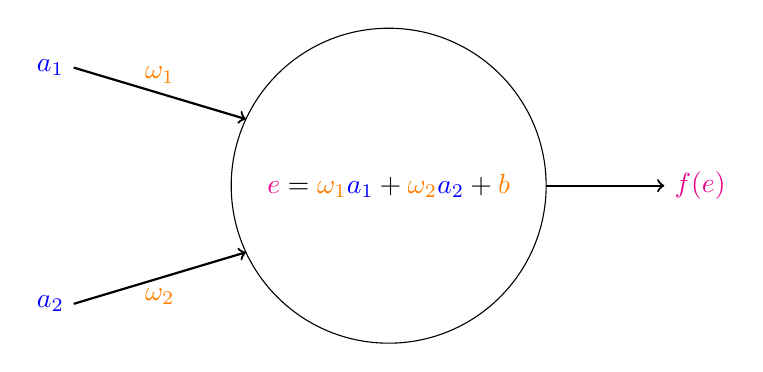
\begin{tikzpicture}[shift={(0,0)}]
	\draw (5,5) circle[radius=2];
	
	% Calculate the coordinates on the circle's circumference
	\pgfmathsetmacro\arrowOneX{5 + cos(155) * 2} % 45 degrees angle
	\pgfmathsetmacro\arrowOneY{5 + sin(155) * 2}
	
	\pgfmathsetmacro\arrowTwoX{5 + cos(-155) * 2} % 135 degrees angle
	\pgfmathsetmacro\arrowTwoY{5 + sin(-155) * 2}
		
	\draw[->, thick] (1,6.5) -- (\arrowOneX, \arrowOneY) node[pos=0.5,above] {$\textcolor{orange}{\omega_1}$};
	\draw (1,6.5) node[left] {$\textcolor{blue}{a_1}$};
	\draw[->, thick] (1,3.5) -- (\arrowTwoX, \arrowTwoY) node[pos=0.5,below] {$\textcolor{orange}{\omega_2}$};
	\draw (1,3.5) node[left] {$\textcolor{blue}{a_2}$};
	\node at (5,5) {$\textcolor{magenta}{e} = \textcolor{orange}{\omega_1}\textcolor{blue}{a_1} + \textcolor{orange}{\omega_2}\textcolor{blue}{a_2} + \textcolor{orange}{b}$};	
	\draw[->, thick] (7,5) -- (8.5,5) node[right] {$\textcolor{magenta}{f(e)}$};
	
	
\end{tikzpicture}